\begin{graphicspathcontext}{{./chapters/simulation/examples/imgs/},{./chapters/simulation/examples/imgs/auto/},\old}

\sidecite{Buisson2014b}
\begin{frame}{Overview of the Hybrid Environment Model}
	\begin{itemize}
	\item Different points of view on the Environment
	\item Distinction between navigation and perception
	\item \emph{Hybrid approach: the HEDGE Graphe, and a 2D/3D tree-based space}
	\end{itemize}
	\begin{center}
		\includegraphics[width=.75\linewidth]{3d_umlhedge}
	\end{center}
\end{frame}

\sidecite{Buisson2014b}
\figureslide{Modeling with a Graph}{3d_hedge4}

\sidecite{Buisson2014b}
\figureslide{Distinction between Navigation and Perception}{3d_overview_npgraph}

\sidecite{Buisson2014b}
\begin{frame}{Nodes in the Environment Graph}
	\begin{block}{Types of nodes}
		\begin{description}
		\item[Corridor] zone with a general direction (roads, corridors\dots)
		\item[Place] spatial zone that corresponds to an open space
		\item[Junction] zone that permits to connect nodes together
		\end{description}
	\end{block}
	\begin{center}
		\includegraphics[width=.6\linewidth]{3d_voxelia_simulate_node_overview}
	\end{center}
\end{frame}

\sidecite{Buisson2014b}
\begin{frame}[t]{Corridor}
	\begin{columns}
		\begin{column}[t]{.6\linewidth}
			\begin{block}{Definition}
			\smaller
			\begin{itemize}
			\item Sequence of shapes: $\langle s_0,s_1\dots\rangle$
			\item $s_i = \langle c_i^{left}, c_i^{right}, c_i^{entry}, c_i^{exit}, t_i\rangle$
			\item $c_i^\alpha$: side of the shape, $t_i$: tangent
			\item $\square\begin{pmatrix}
				(s_i \cap s_{k\neq i})=\emptyset\;\wedge\;c_i^{left} \| c_i^{right}\\
				\wedge\;c_{i-1}^{exit}=c_{i}^{entry}\;\wedge\;c_{i+1}^{entry}=c_{i}^{exit}
				\end{pmatrix}$
			\item $c_0^{entry}$ and $c_n^{exit}$ are connectable to one node each
			\end{itemize}
			\end{block}
			\begin{block}{Building}
			\begin{enumerate}
			\item Extrusion of a spline or a path
			\item Discretization such that $t_j.t_i\le\epsilon$
			\end{enumerate}
			\end{block}
		\end{column}
		\begin{column}[t]{.4\linewidth}
			\raisebox{-\height}{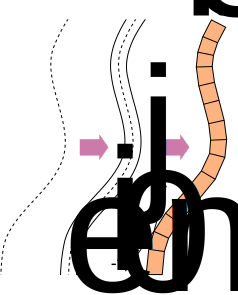
\includegraphics{3d_construct_corridor}}
		\end{column}
	\end{columns}
\end{frame}

\sidecite{Buisson2014b}
\begin{frame}{Open Place}
	\begin{columns}
		\begin{column}[t]{.75\linewidth}
			\begin{block}{Definition}
			\smaller
			\begin{itemize}
			\item Set of triangles forming a bounded 2D manifold: $\{ t_0,t_1\dots\}$
			\item $t_i = \{ s_i^0, s_i^1, s_i^2 \}$, $s_i^\alpha$ = triangle side
			\item $\square (t_i \cap t_{k\neq i})=\emptyset$
			\item $\square \left(\nexists k,b / s_i^a = s_{k\neq i}^b \Rightarrow s_i^a \in B\right)$
			\item $B$: sequence of sides that forms the bounds of the place, such that the first segment is connected to the last segment
			\item Each element of $B$ may be connectable to many nodes, without overlapping
			\end{itemize}
			\end{block}
		\end{column}
		\begin{column}[t]{.25\linewidth}
			\raisebox{-\height}{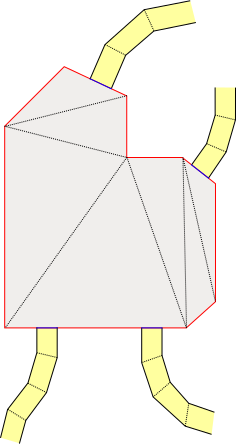
\includegraphics{3d_overview_place}}
		\end{column}
	\end{columns}
\end{frame}

\sidecite{Buisson2014b}
\begin{frame}{Junction}
	\begin{columns}
		\begin{column}[t]{.6\linewidth}
			\begin{block}{Definition}
			Specialization of a place, in which:
			\begin{itemize}
			\item $|B| = 4$
			\item $\forall b \in B$, the connected nodes are always the junction and a set of corridors
			\end{itemize}
			\end{block}
		\end{column}
		\begin{column}[t]{.35\linewidth}
			\raisebox{-\height}{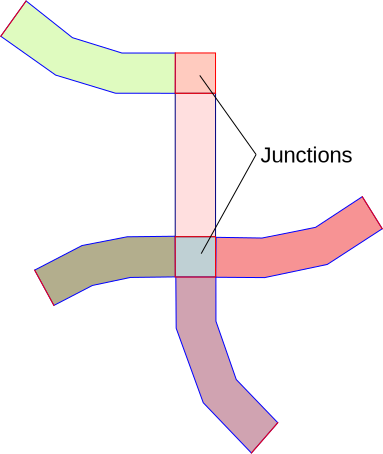
\includegraphics{3d_overview_junction}}
		\end{column}
	\end{columns}
\end{frame}

\sidecite{Buisson2014b}
\begin{frame}[t]{Connectors}
	\begin{description}
	\item[Standard connector] connects two nodes
	\item[Lane-change connector] enables to connect two adjacent corridors
	\item[Conflict connector] add a perception link between to overlapping nodes
	\end{description}
	\begin{columns}
		\begin{column}[t]{.6\linewidth}
			\raisebox{-.5\height}{\includegraphics{3d_voxelia_simulate_connector_overview}}
		\end{column}
		\begin{column}[t]{.25\linewidth}
			\raisebox{-.5\height}{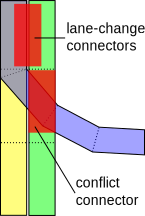
\includegraphics{3d_overview_conflict_connector}}
		\end{column}
	\end{columns}
\end{frame}

\sidecite{Buisson2014b}
\begin{frame}{Simulation of the Urban Infrastructure of Belfort}
	\begin{enumerate}
	\item Realistic behaviors: use for infrastructure design by experts and stakeholders.
	\vspace{2em}
	\item Quick respond to change requests: less than 2 working days for (re-)designing the simulation environment and a scenario.
	\vspace{2em}
	\item Realtime: use during public meetings with citizens.
	\end{enumerate}
\end{frame}

\sidecite{Buisson2014b}
\figureslide{Modeling of a Cross-road from a Map}{3d_hedge1}

\sidecite{Buisson2014b}
\begin{frame}[t]{{Automatic Generation} of the Graph}
	\begin{columns}
		\begin{column}{.4\linewidth}
			\begin{itemize}
			\item 56 nodes
			\item 264 links
				\begin{itemize}
				\item 156 perception links
				\item 108 navigation links
				\end{itemize}
			\end{itemize}
		\end{column}
		\begin{column}{.55\linewidth}
			\includegraphics{3d_hedge2}
		\end{column}
	\end{columns}
	\includegraphics{3d_hedge3}
\end{frame}

\sidecite{Buisson2014b}
\begin{frame}[t]{Video (1/2)}
	\begin{center}
		\embeddedvideo[width=.75\linewidth]{./videos/simulation/pedestrians_place_arme_belfort.avi}{pedestrians_place_arme_belfort}
	\end{center}
	\begin{center}
	\tiny These videos were realized on the SIMULATE\textup{\regmark} tool \copyright Voxelia S.A.S
	\end{center}
\end{frame}

\sidecite{Buisson2014b}
\begin{frame}[c]{Video (2/2)}
	\begin{center}
		\embeddedvideo[width=.75\linewidth]{./videos/simulation/pedestrians_rabin_belfort.avi}{pedestrians_rabin_belfort}
	\end{center}
	\begin{center}
	\tiny These videos were realized on the SIMULATE\textup{\regmark} tool \copyright Voxelia S.A.S
	\end{center}
\end{frame}

\end{graphicspathcontext}
